\chapter{Introducción\label{sec:introduccion}}

Desde el principio de los tiempos la humanidad se ha esforzado por comprender el entorno que le rodea, aprender de él y usarlo en su propio beneficio para conseguir así hacer su vida más fácil. Por el momento hemos conseguido hacer volar aviones gracias a la observación de los pájaros o crear sistemas de sonar que se asemejan al sistema que utilizan los murciélagos para orientarse. Pero irónicamente, a pesar del esfuerzo invertido, nuestro propio cuerpo sigue albergando secretos que desentrañar que podrían facilitarle la vida a un gran número de personas.

El estudio del \textbf{cuerpo humano} ha sido uno de los temas más polémicos y que más ha evolucionado desde que hay registro. Aunque al comienzo estuvo muy marcado por la superstición y la religión, achacando la mayoría de las dolencias y efectos sanadores a la magia, con el paso del tiempo aparecieron personas como Hipócrates y Aristóteles que fueron capaces de aportar un nuevo enfoque basado en la \textbf{observación y estudio} de lo que les rodeaba, asentando unas bases que, posteriormente, serían aprovechadas y mejoradas hasta convertirse en lo que conocemos hoy en día como \textbf{método científico}.

El proceso de descubrimiento del funcionamiento del cuerpo humano ha seguido diferentes fases a lo largo de la historia. Comparar el cuerpo humano con animales fue uno de los primeros pasos para descubrir cómo estábamos formados por dentro. Posteriormente, aprovechando los cuerpos de personas ya fallecidas se estudió la anatomía humana, permitiendo así crear mapas y dibujos de la estructura del cuerpo humano y sus órganos bastante detallados.

\begin{figure} [H]
    \centering
    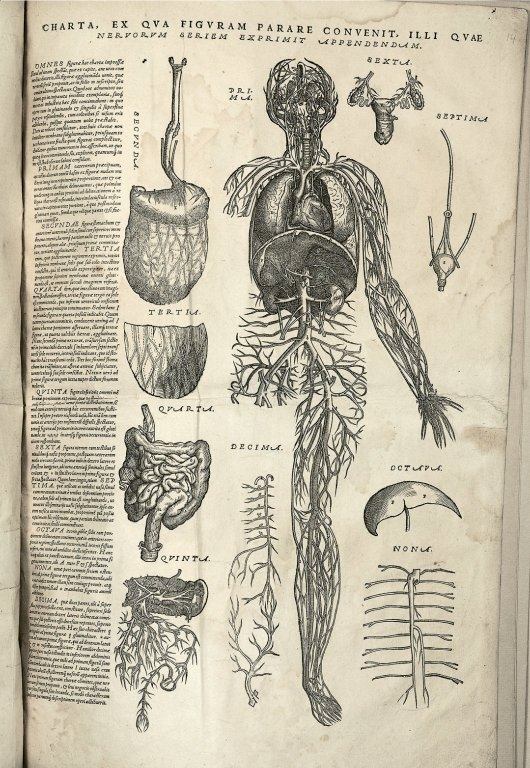
\includegraphics[width=0.25\textwidth]{Anatomia}
    \caption{Ejemplo de anatomía humana.}
    \label{fig:Anatomia}
\end{figure}

Pese a todo, estudiar cuerpos inertes tiene sus limitaciones de modo que durante un tiempo se realizaron vivisecciones para poder comprender mejor como funcionaban todos aquellos órganos, músculos y nervios que ya habían visto con anterioridad. Con el paso del tiempo este sistema fue descartado ya que es una práctica que ponía en peligro la vida del sujeto, haciéndolo pasar por una experiencia terrible en el mejor de los casos.

En la actualidad, gracias al conocimiento acumulado de muchos años y a los \textbf{avances en otros campos de la ciencia}, se han desarrollado dispositivos y técnicas que permiten el \textbf{estudio en vivo} del comportamiento del cuerpo humano de \textbf{forma no invasiva}. Es posible utilizar \textbf{ecografías} para ver el estado del corazón, radiografías para diagnosticar un hueso roto e incluso técnicas más avanzadas como la \textbf{medicina nuclear} que permiten saber que partes del cerebro se activan frente a determinados estímulos sin necesidad de interactuar físicamente con él.

Si bien todas las técnicas anteriores han supuesto auténticos hitos en la medicina moderna y han permitido diagnosticar un gran número de enfermedades así como mejorar la calidad de vida de muchas personas, la mayoría presenta inconvenientes que hacen improbable su uso a nivel personal o docente debido al tamaño de los equipos necesarios para su realización o el coste muy elevado del procedimiento (sin contar con el conocimiento necesario para la realización correcta de la prueba).

Teniendo en mente esta problemática se han desarrollado dispositivos capaces de medir pequeñas las variaciones de voltaje que se producen en el interior de nuestro cuerpo haciendo uso de unos dispositivos denominados \textbf{electrodos}.
\\De esta forma es posible, con un \textbf{coste muy reducido} y un equipamiento relativamente asequible, conseguir inferir que procesos químicos y físicos se están produciendo en el interior de nuestro cuerpo.

Haciendo uso de este sistema se pueden obtener registros sobre diferentes actividades acaecidas en el cuerpo humano. En función del origen de estas señales reciben los siguientes nombres: electrocardiograma (ECG) para las señales originadas por las contracciones del corazón; electromiograma (EMG) para las generadas en los músculos; electroencefalograma (EEG) para aquellas generadas en el cerebro, etc.

\begin{figure} [H] %this figure will be at the center
    \centering
    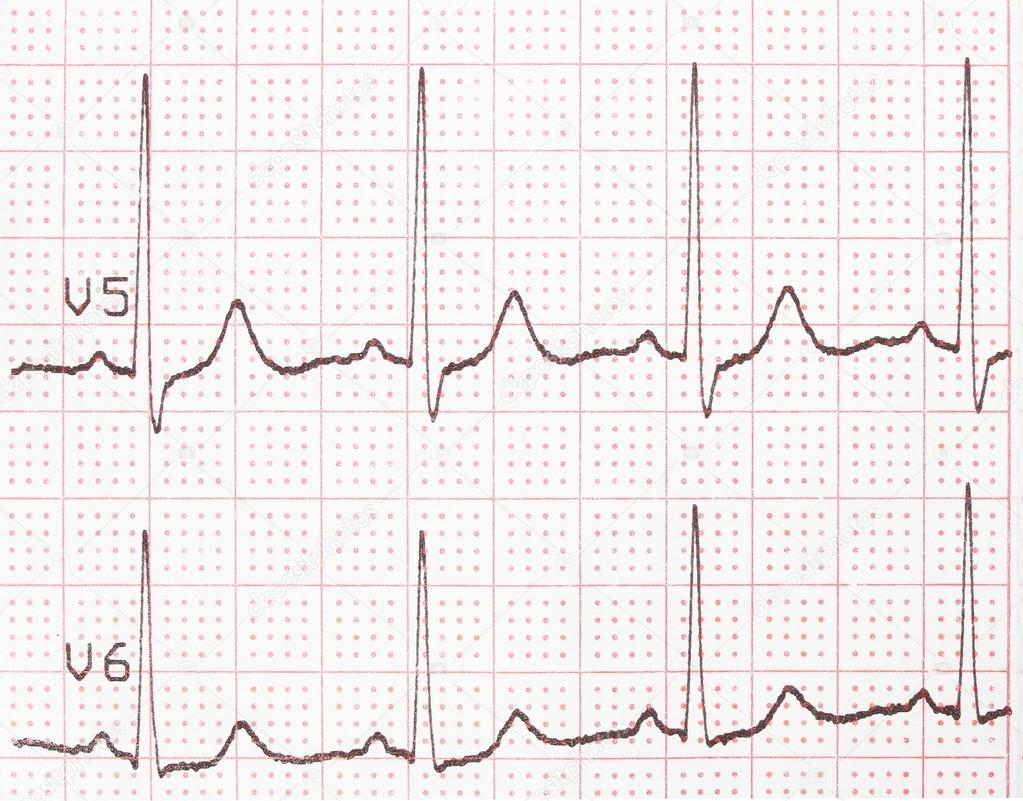
\includegraphics[width=7.5cm]{ECG}
    \caption{Ejemplo de ECG}
    \label{fig:ECG}
\end{figure}

\section{Alcance y estructura del proyecto}
El \textbf{objetivo de este proyecto} es realizar un sistema capaz de captar señales de electroencefalogramas (EEG) manteniendo una buena \textbf{relación prestaciones/coste}. El sistema estará compuesto de dos tarjetas, una de acondicionamiento y de adquisición de datos basada en el circuito integrado ADS1299 y otra de \textbf{procesamiento y transmisión} de dicha información. Esta última es el objetivo del presente proyecto. La plataforma de procesamiento estará basada en un procesador de altas prestaciones, dispondrá de interfaces \textbf{Wifi}, \textbf{Bluetooth} y \textbf{almacenamiento USB} para la transmisión y almacenamiento de los datos respectivamente. 

En la primera fase del proyecto se seleccionará el microcontrolador más adecuado entre los existentes en el mercado analizando características como: capacidad de procesado, interoperación con otros dispositivos, prestaciones...
\\Se compararán los microcontroladores ofrecidos por los distintos fabricantes (ST Microelectronics, Texas instruments, etc) y finalmente, se escogerá aquel que mejor se adecúe a las necesidades del proyecto siendo los principales candidatos los de la familia \textbf{ARM-M4 STM32F4x} por su excelente relación prestaciones-coste.
\\Se valorará también la posibilidad de utilizar diferentes herramientas para la programación del microcontrolador y las alternativas \textit{\gls{Open Source}} en caso de existir.

Una vez completado el diseño eléctrico de la tarjeta se procederá al \textbf{diseño de la \acrshort{PCB} equivalente}, la cual se implementará utilizando \textbf{tecnología \acrshort{SMT}} en su mayor parte. Para el diseño de la placa se utilizará KiCad por las numerosas ventajas que presenta al ser software libre y la gran cantidad de información que se puede encontrar sobre el funcionamiento del mismo.
Tras depurar la \acrshort{PCB}, se implementará un sencillo \textbf{firmware} que permita testear el hardware diseñado y hacer una adquisición básica utilizando la tarjeta desarrollada junto con la de adquisición cedida por parte de Nerea Urrestarazu.

Adicionalmente se pondrá en marcha un \textbf{programa para el ordenador} basado en LabView donde presentar los datos recibidos.

\section{Base teórica\label{sec:Base_teorica}}

% Documentación interesante para esta sección: 
% http://slideplayer.es/slide/3413933/

Antes de empezar a desarrollar el dispositivo ya mencionado es indispensable realizar una investigación previa del origen de las señales que se quieren adquirir, haciendo especial hincapié en las características de las mismas\footnotemark{}.

\footnotetext{El contenido de esta sección se ha obtenido en su mayor parte de las diapositivas de la asignatura de Señales e Imágenes Médicas impartida por Jose Javier Serrano Olmedo \cite{apuntes}}

\begin{wrapfigure}[14]{R}{8cm}
    \centering
    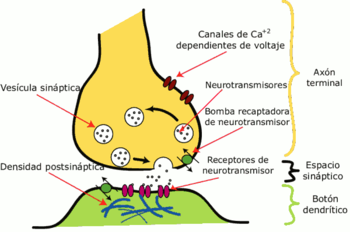
\includegraphics[width=8cm]{Intro_neuronas}
    \caption{Sinapsis neuronal \cite{wikipedia}}
    \label{fig:Intro_neuronas}

\end{wrapfigure}
En el cerebro se realizan \textbf{millones de conexiones} diarias entre las células que la conforman. Dichas células reciben el nombre de \textbf{neuronas}. La comunicación entre ellas se realiza mediante el \textbf{intercambio de neurotransmisores}, proceso que recibe el nombre de sinapsis y que provoca una corriente eléctrica de mayor o menor intensidad que permite la inhibición o activación de las distintas neuronas. 

La suma de todas las corrientes eléctricas conforma lo que se denomina \textbf{actividad bioeléctrica cerebral}. Mediante el uso de sensores es posible medirla y representarla.

Las señales del \acrshort{EEG} dependen del estado de consciencia del usuario y se pueden clasificar en función de su amplitud y frecuencia. Las principales ondas son las siguientes:

\begin{itemize}
\item\textbf{Ondas delta} (hasta 3.5 Hz). Término introducido por W. G. Walter en 1937 para describir a estas ondas de baja frecuencia y alta intensidad (unos centenares de $\mu$V). Tienen lugar en niños de corta edad y en adultos sólo en estado de sueño profundo, inconsciencia o situaciones que aumenten la presión intercraneal como tumores cerebrales.
\end{itemize}
\begin{figure} [H]
    \centering
    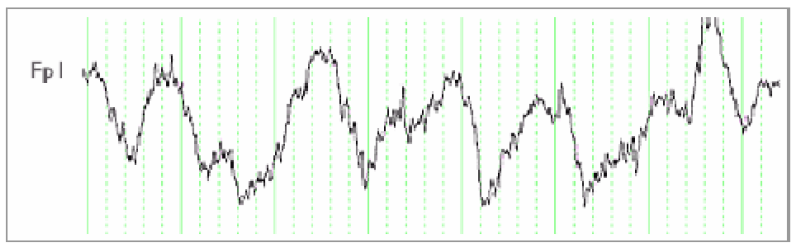
\includegraphics[width=13cm]{ondas_delta}
    \caption{Ondas delta \cite{apuntes}}
    \label{fig:ondas_delta}
\end{figure}

\clearpage

\begin{itemize}
\item\textbf{Ondas theta} (3.5 - 7.5 Hz). Término también Walter aunque mucho más tarde, en 1953. Estas ondas de amplitud inferior a 20 $\mu$ se dan durante el proceso de maduración en toda la corteza cerebral, aunque predomina en la región occipital y temporal y es más rápida en la zona frontal. Dominante en niños entre 5 y 7 años y aún quedan rastros en la juventud. En adultos y adolescentes se asocia a situaciones emocionales y pensamientos de tipo creativo, a estrés o a desordenes psíquicos.
\end{itemize}
\begin{figure} [H]
    \centering
    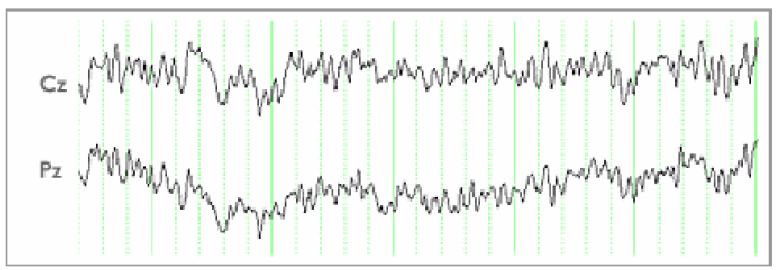
\includegraphics[width=13cm]{ondas_theta}
    \caption{Ondas theta \cite{apuntes}}
    \label{fig:ondas_theta}
\end{figure}

\begin{itemize}
\item\textbf{Ondas alfa} (7.5 - 12.5 Hz). Berger utilizó el término de ritmo alfa para ráfagas de 20-100 $\mu$V de amplitud y gran periodicidad a esas frecuencias predominantes sobre la región occipital pero que aparecen en todo el córtex. Se asocian a estados de relajación, de inactividad y son muy patentes en ausencia de estímulos visuales. Existe mucha variabilidad interpersonal en el ritmo alfa.
\end{itemize}
\begin{figure} [H]
    \centering
    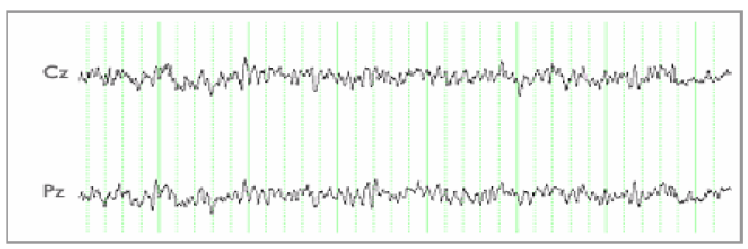
\includegraphics[width=13cm]{ondas_alfa}
    \caption{Ondas alfa \cite{apuntes}}
    \label{fig:ondas_alfa}
\end{figure}

\begin{itemize}
\item\textbf{Ondas beta} (12.5 - 30 Hz). Estas señales de pequeña amplitud, por debajo de 20$\mu$V, son bastante comunes y predominan durante la edad adulta. Suele dividirse en beta baja, beta media y beta alta. El ritmo beta bajo se suele localizar en los lóbulos frontal y occipital y los otros dos están menos localizados. Más irregular que el ritmo alfa, se asocia a actividad psicofísica, estados de agitación, alerta o la actividad mental que se realiza en la resolución de problemas.
\end{itemize}
\begin{figure} [H]
    \centering
    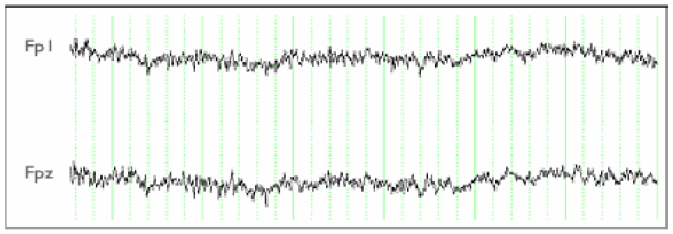
\includegraphics[width=13cm]{ondas_beta}
    \caption{Ondas beta \cite{apuntes}}
    \label{fig:ondas_beta}
\end{figure}

\begin{itemize}
\item\textbf{Ondas gamma} (12.5 - 30 Hz). Esta banda tiene un pico de resonancia, similar a los ritmos alfa, cercano a 40Hz al que se da el nombre de épsilon que se asocia a actividad mental abstracta que interviene en percibir como único por ejemplo el olor, los rasgos de la cara, la personalidad y la voz de una persona. Actualmente hay quien habla de ondas de frecuencias superiores a 50 Hz, son las hipergamma hasta 100 Hz y las lambda hasta 200 Hz, se dice aparecen en los monjes tibetanos en estados de meditación profunda
\end{itemize}

Para la realización de un electroencefalograma existe una disposición estándar en la colocación de los sensores denominada \textbf{sistema 10-20}. Se trata de un sistema internacional que indica la posición en la que se deben colocar los electrodos para una medición del \acrshort{EEG}.  Este sistema separa el cuero cabelludo en torno a un eje Z, colocando los electrodos numerado de manera par a la derecha y los impares a la izquierda (tal y como se puede ver en la figura \ref{fig:colocacion_electrodos}).

\begin{figure} [H]
    \centering
    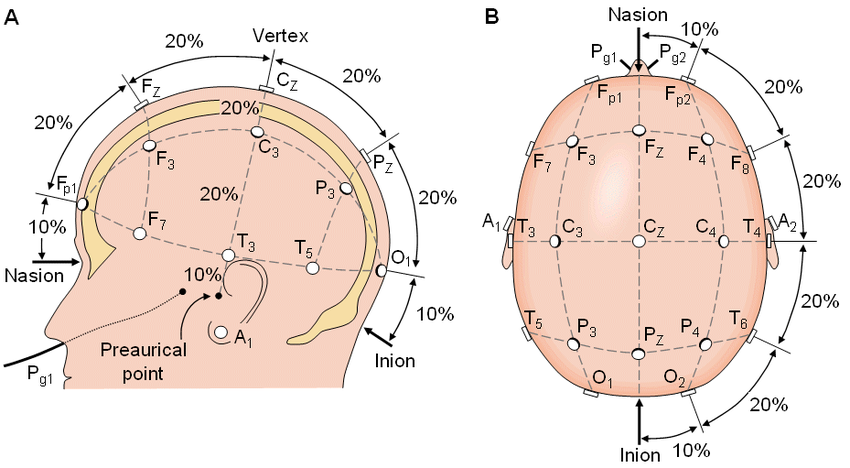
\includegraphics[width=12cm]{colocacion_electrodos}
    \caption{Esquema de colocación de los electrodos \cite{apuntes}}
    \label{fig:colocacion_electrodos}
\end{figure}

\clearpage

\section{Tipos de electrodos\label{sec:Tipos_Electrodos}}

Los electrodos hacen la función de interfaz adaptadora entre los distintos medios por los que se transmiten las señales permitiendo así obtener una señal de mejores características. Este es un funcionamiento similar al de los huesos del oído, pues estos adaptan la señal acústica para que la señal percibida en la coclea tenga unas características determinadas. El funcionamiento de la mayoría de los dispositivos de adquisición de señales en el cuerpo humano depende de estos elementos y hacen uso de dos tipos principales, de trabajo y auxiliar.
\\El electrodo denominado ``de trabajo'' (\textit{working electrode}) es el que adquiere la señal de interés. El otro, denominado auxiliar, es el encargado de crear una referencia. El esquema de la figura \ref{fig:electrodos} muestra un esquema básico de funcionamiento:

\begin{figure} [h]
    \centering
    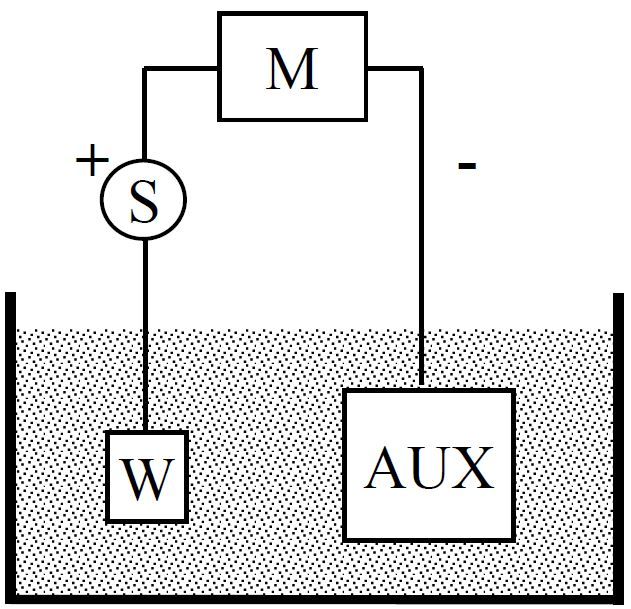
\includegraphics[width=7cm]{electrodos}
    \caption{Electrodos de en un sistema de adquisición \cite{apuntes}}
    \label{fig:electrodos}
\end{figure}

En función del método utilizado por el electrodo para hacer la interfaz con el cuerpo humano estos electrodos se pueden dividir en dos grandes grupos, cada uno con sus ventajas e inconvenientes. 

\subsection{Electrodos húmedos\label{sec:Elec_humedos}}

Los electrodos húmedos se caracterizan por utilizar algún material acuoso para realizar la interfaz entre el dispositivo y el cuerpo humano. Al estar conformados por varios materiales de distinta naturaleza estos electrodos suelen ser de construcción compleja. La figura \ref{fig:electrodo_humedo_2} muestra el esquema de un electrodo húmedo.

\begin{figure} [H]
    \centering
    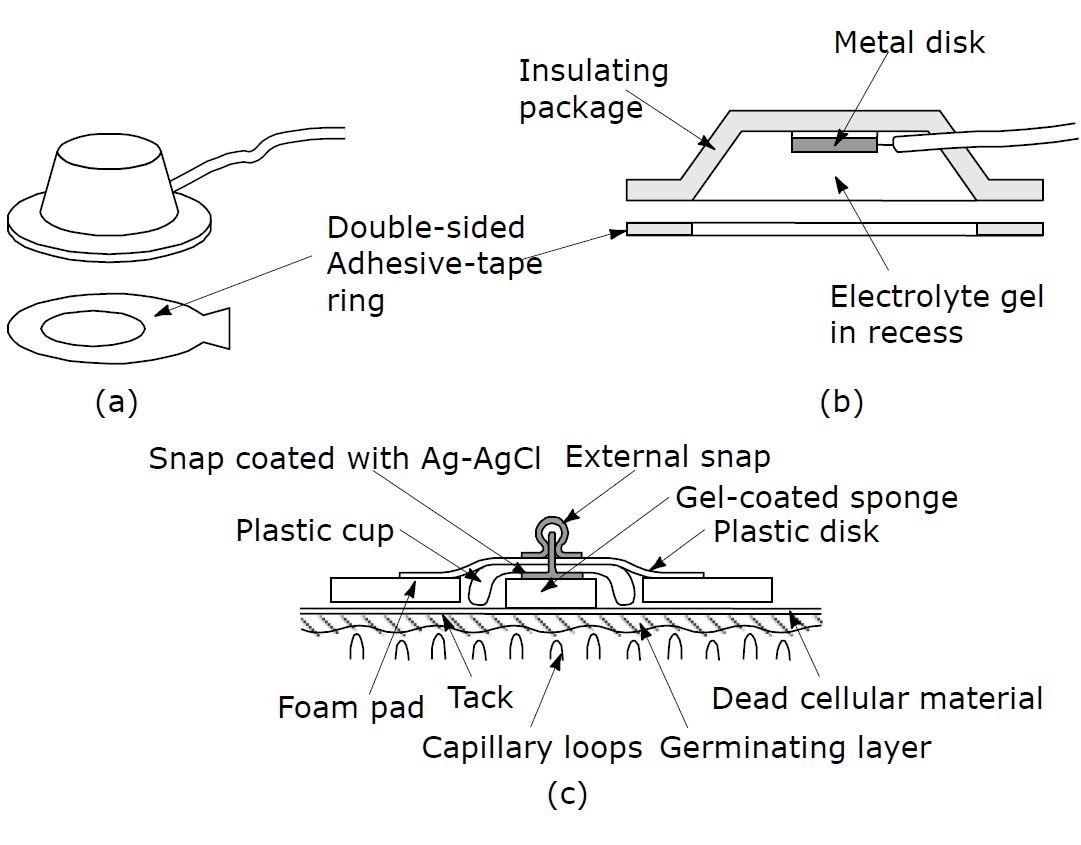
\includegraphics[width=10cm]{electrodo_humedo_2}
    \caption{Esquema de un electrodo húmedo \cite{apuntes}}
    \label{fig:electrodo_humedo_2}
\end{figure}

Estos dispositivos suelen dar muy buen resultado, consiguiendo señales con una buena amplitud y \acrshort{SNR} pero el material utilizado como interfaz suele ser desechable lo que obliga a usar electrodos de usar y tirar o a tener que dedicar mucho tiempo en la preparación y rellenado con gel de la cámara interior del dispositivo. Además, desde el punto de vista de la comodidad del usuario, la utilización de electrodos húmedos puede resultar incómoda al obligarlo a lavar la zona antes y después de su utilización.

La figura \ref{fig:electrodo_humedo_1} muestra un ejemplo de adquisición de \acrshort{EEG} utilizando electrodos húmedos.

\begin{figure} [h]
    \centering
    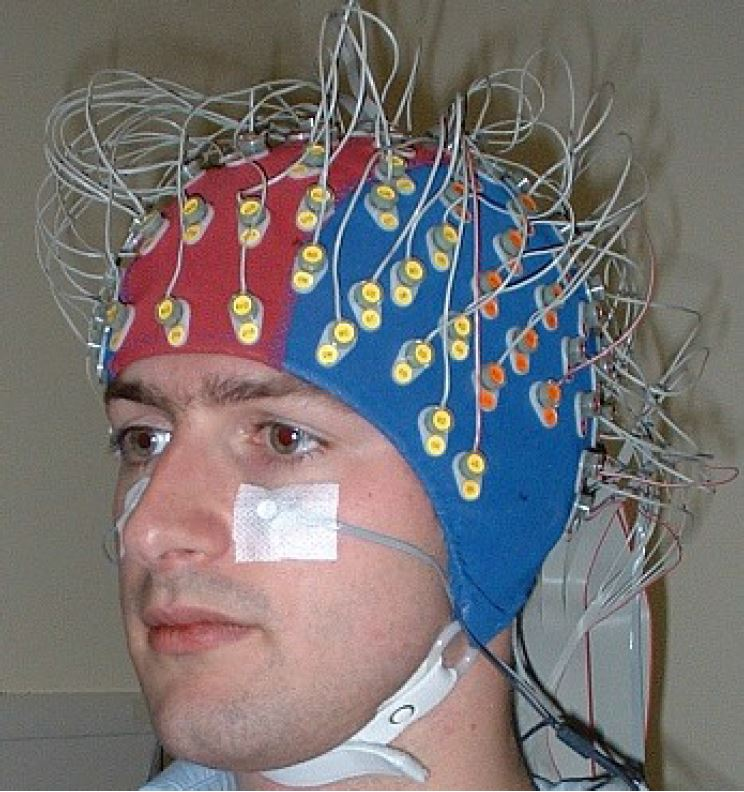
\includegraphics[width=7cm]{electrodo_humedo_1}
    \caption{Medida de un EEG usando electrodos húmedos \cite{apuntes}}
    \label{fig:electrodo_humedo_1}
\end{figure}

\clearpage

\subsection{Electrodos secos\label{sec:Elec_secos}}

Los electrodos secos utilizan materiales sólidos cuya interacción con el cuerpo humano resulta favorable. Al realizar una interfaz con materiales sólidos las señales se transmiten con mayor dificultad, pero este sistema resulta mucho más cómodo para el usuario y los electrodos son de fabricación más sencilla y reutilizables. La figura \ref{fig:electrodo_seco} muestra una representación 3D de un electrodo seco (derecha) y un electrodo seco real junto con sus correspondientes conectores (izquierda).

\begin{figure} [h]
    \centering
    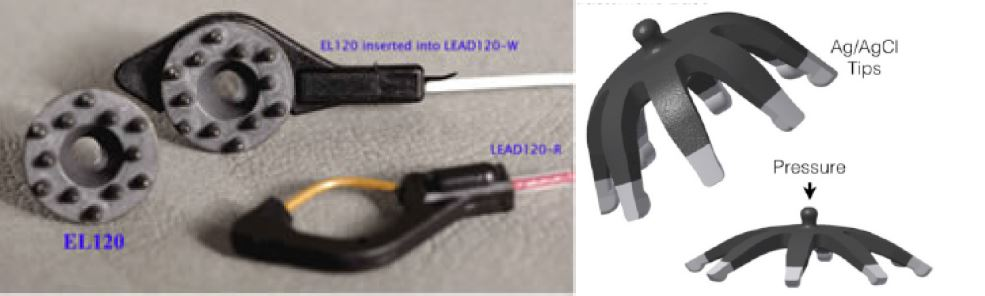
\includegraphics[width=13cm]{electrodo_seco}
    \caption{Electrodo seco real(izquierda) y representación 3D (derecha) \cite{apuntes}}
    \label{fig:electrodo_seco}
\end{figure}

Por comodidad durante la realización de este proyecto se utilizarán principalmente electrodos secos pero la posibilidad de usar electrodos húmedos se mantendrá, pues la utilización de unos u otros afecta al usuario final y a los resultados pero apenas al equipo encargado de su adquisición.
